\clearpage

\begin{figure}[h]
  \section{\ruby{解答}{かいとう}例}

  図{~\ref{fig:48}はしゅみの\ruby{紹介}{しょうかい}のホームページの例です。HTMLファイルは01フォルダのsample3.htmlです。参考に\ruby{確認}{かくにん}しましょう。}\\
  図{~\ref{fig:49}は学校\ruby{紹介}{しょうかい}のホームページの例です。HTMLファイルは01フォルダのsample2.htmlです。参考に\ruby{確認}{かくにん}しましょう。}\\
  図{~\ref{fig:50}は\ruby{時間割}{じかんわり}表の例です。HTMLファイルは01フォルダのsample1.htmlです。参考に\ruby{確認}{かくにん}しましょう。}\\

  \centering
  \begin{minipage}{0.45\textwidth}
    {\upshape
      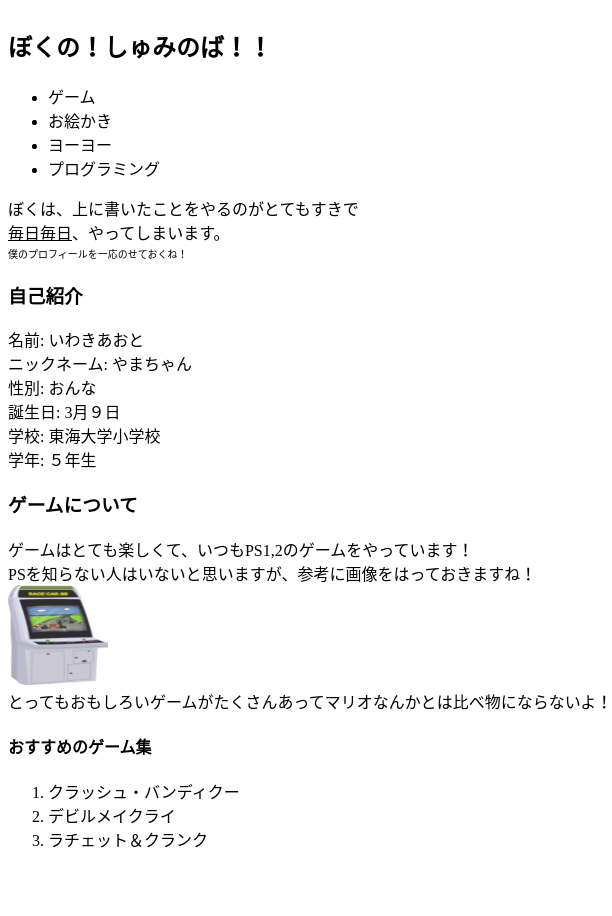
\includegraphics[width=0.9\linewidth]{text01-img/textbook-img209.png}
      \caption{\ruby{趣味}{しゅみ}ホームページサンプル}\label{fig:48}
    }
  \end{minipage}
  \begin{minipage}{0.45\textwidth}
    {\upshape
      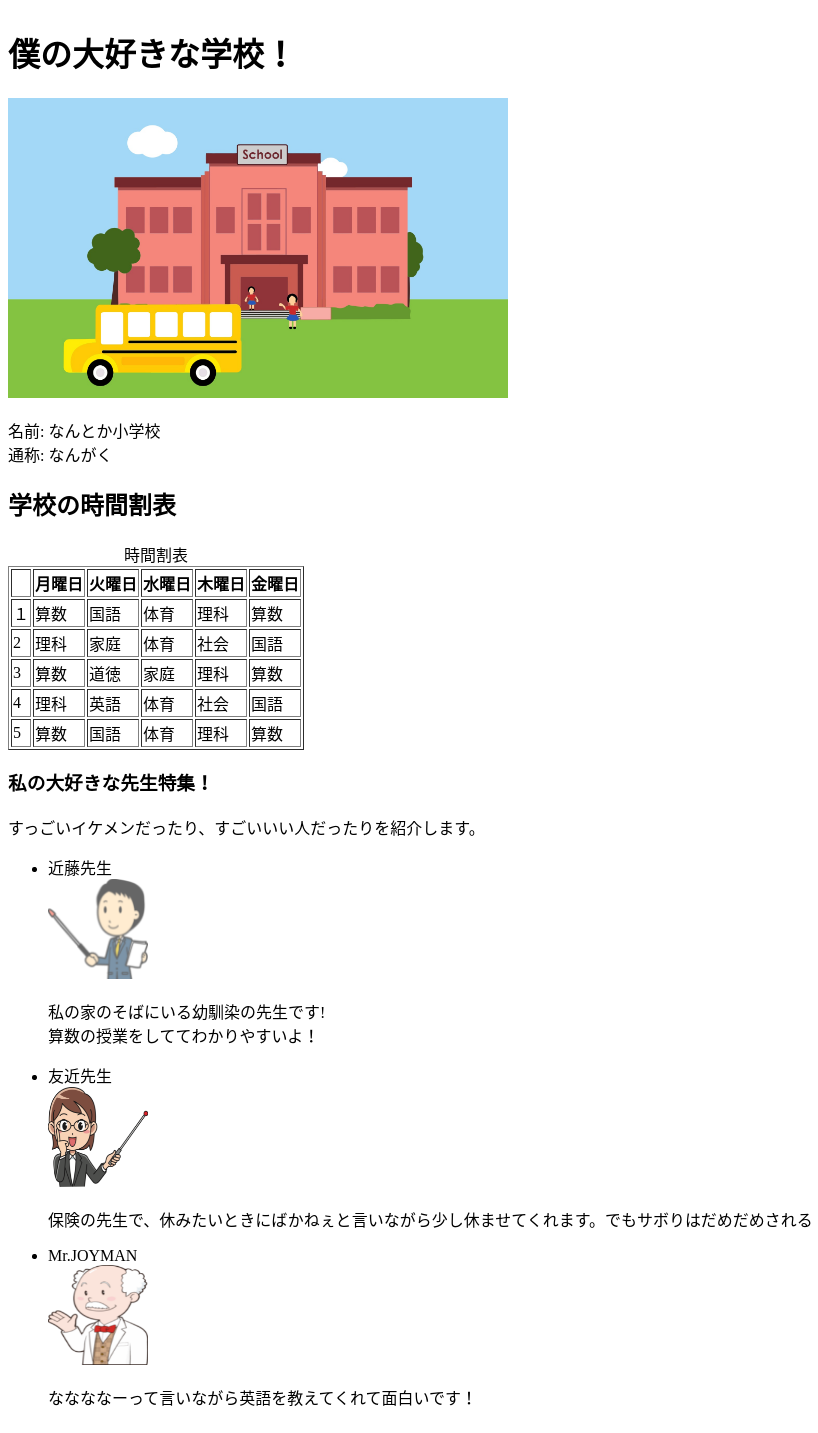
\includegraphics[width=0.9\linewidth]{text01-img/textbook-img210.png}
      \caption{学校\ruby{紹介}{しょうかい}ホームページサンプル}\label{fig:49}
    }
  \end{minipage}

  \centering
  \begin{minipage}{0.43\textwidth}
    {\upshape
      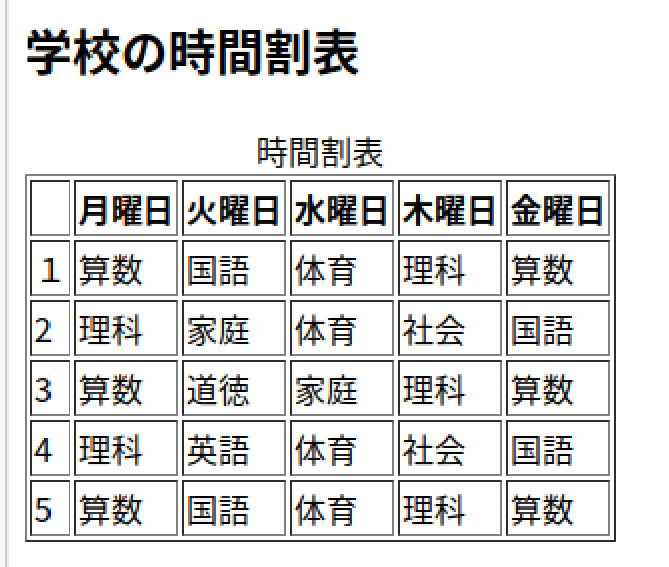
\includegraphics[width=\linewidth]{text01-img/textbook-img211.png}
      \caption{\ruby{時間割}{じかんわり}表サンプル}\label{fig:50}
    }
  \end{minipage}  
\end{figure}

\clearpage
\subsection{\bfseries 問題の答え}

問題の答えをのせてあります。まずは答えをみないで\ruby{解}{と}いていきましょう。\newline
問題の答えがないところは例題とほぼ変わらないためはぶいています。

\subsubsection{\bfseries 問題 1-2 答え}

  (1)×\hspace{2em}(2)×\hspace{2em}(3)○\hspace{2em}(4)×
  % (2)訂正箇所:使用して良い \hspace{2em} 訂正後:使用してはいけない\newline(3)訂正箇所:×\newline(4)訂正箇所:組み合わせが良い\hspace{2em} 訂正後:組み合わせにしないこと\newline

  \subsubsection{\bfseries 問題 1-3 答え}

  (1)○\hspace{2em}(2)×\hspace{2em}(3)×\hspace{2em}(4)○

  \subsubsection{\bfseries 問題 1-4 答え}

  (1)○\hspace{2em}(2)×\hspace{2em}(3)×\hspace{2em}(4)×

\clearpage

\subsubsection{\bfseries 問題 1-7 答え}

\bigskip


\centering
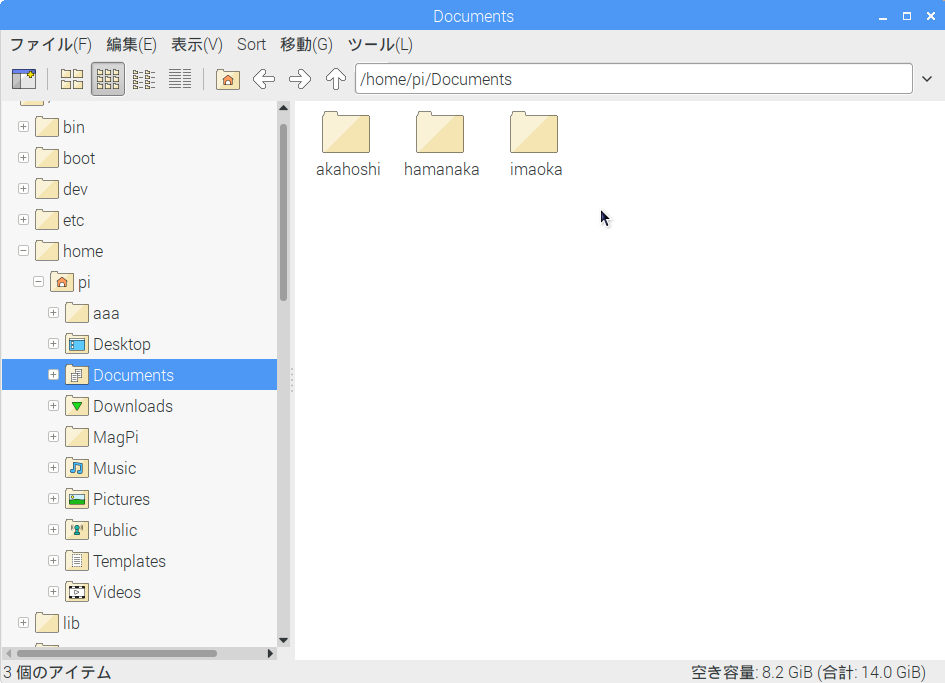
\includegraphics[width=0.65\textwidth]{text01-img/textbook-img212.png}
\flushleft

\bigskip


\bigskip


\bigskip

\subsubsection{\bfseries 問題 1-8 答え}

\bigskip



\centering
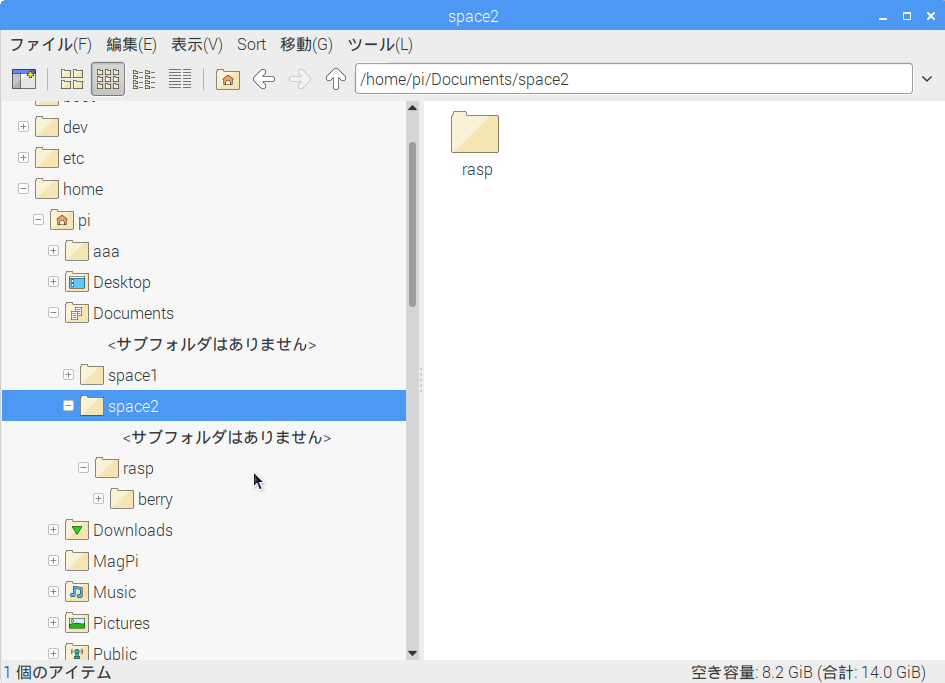
\includegraphics[width=0.65\textwidth]{text01-img/textbook-img213.png}
\flushleft

\clearpage\subsubsection{\bfseries 問題 1-9 答え}


\begin{enumerate}
  \item
        miss\_nameフォルダの上で右クリックしてファイル名の\ruby{変更}{へんこう}をクリック

        \centering
        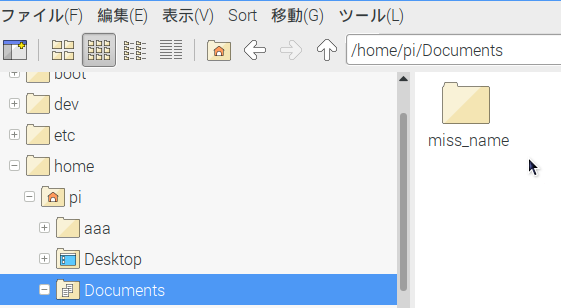
\includegraphics[width=0.6\textwidth]{text01-img/textbook-img214.png}
        \flushleft

  \item success\_nameに\ruby{変更}{へんこう}

        \centering
        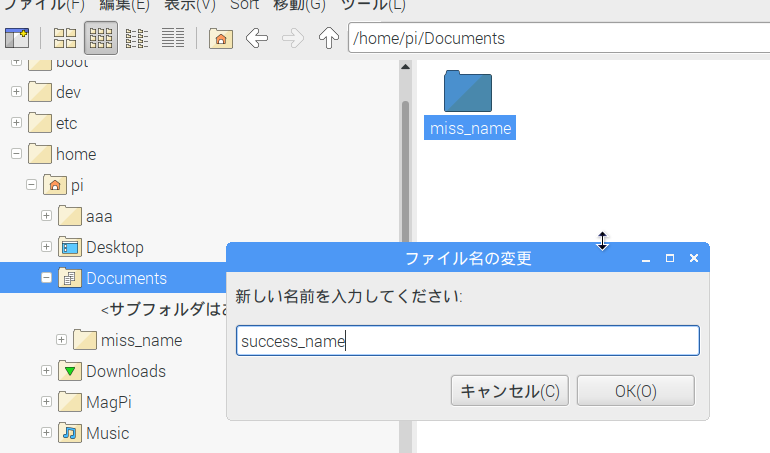
\includegraphics[width=0.6\textwidth]{text01-img/textbook-img215.png}
        \flushleft
  \item success\_nameに\ruby{変更}{へんこう}できました

        \centering
        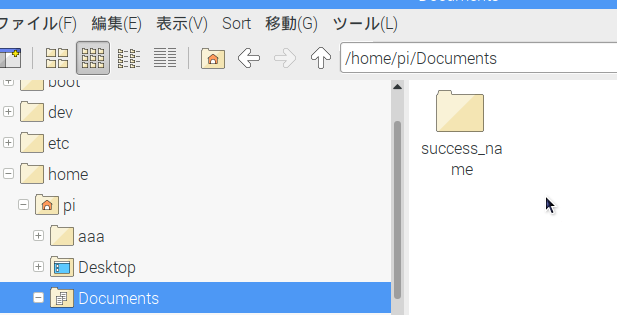
\includegraphics[width=0.6\textwidth]{text01-img/textbook-img216.png}
        \flushleft
\end{enumerate}

\clearpage
\subsubsection{\bfseries 問題 1-10 答え}

shiftキーを\ruby{押}{お}しながら、アルファベットキーを打つと大文字入力になるよ

\centering
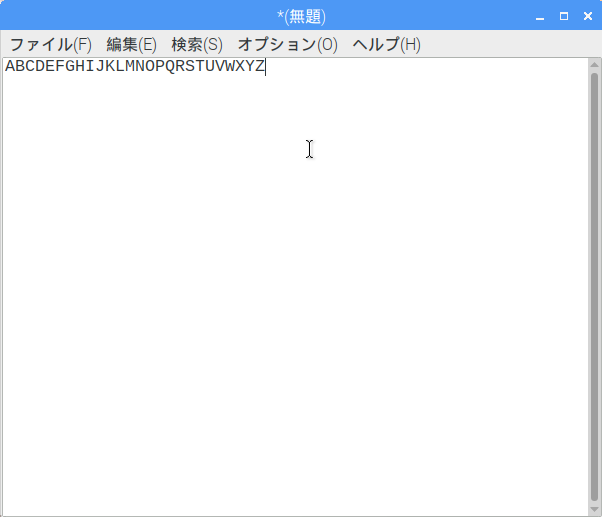
\includegraphics[width=0.6\textwidth]{text01-img/textbook-img217.png}
\flushleft

\clearpage
\subsubsection{\bfseries 問題 1-11 答え}

右上にキーボードマークが出ていることを\ruby{確認}{かくにん}しよう。そのじょうたいで入力しよう。


\bigskip


\centering
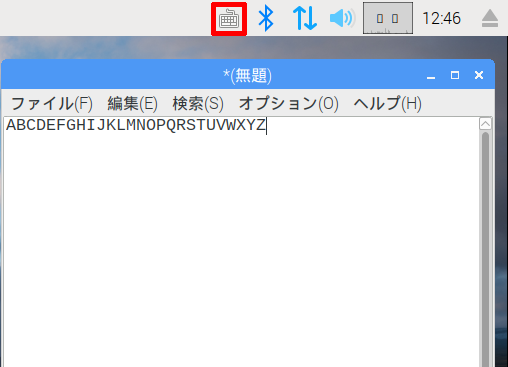
\includegraphics[width=0.6\textwidth]{text01-img/textbook-img218.png}
\flushleft


\bigskip





\centering
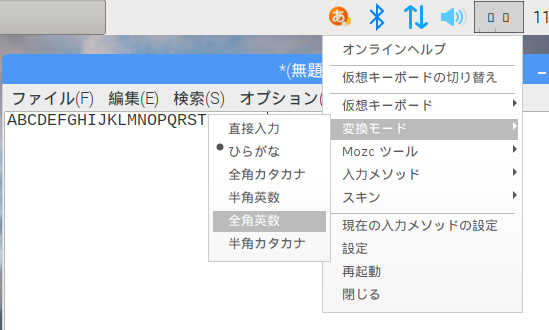
\includegraphics[width=0.6\textwidth]{text01-img/textbook-img219.png}
\flushleft


\bigskip

{\bfseries
  半角大文字でアルファベットの入力を終えたら右上のキーボードマークをクリックし

  「あ」マークにして右クリックし、\ruby{変換}{へんかん}モードから全角英数をクリック}



\bigskip

\bigskip


\centering
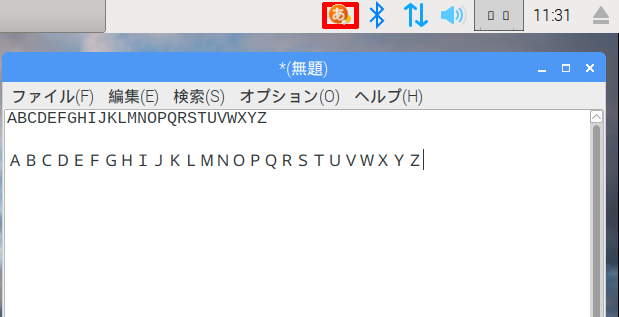
\includegraphics[width=0.6\textwidth]{text01-img/textbook-img220.png}
\flushleft

\bigskip

全角アルファベットを入力しよう。
\clearpage

\subsubsection{\bfseries 問題 1-13 答え}

参考にして、じぶんの好きな\ruby{画像}{がぞう}を\ruby{保存}{ほぞん}しよう。

\centering
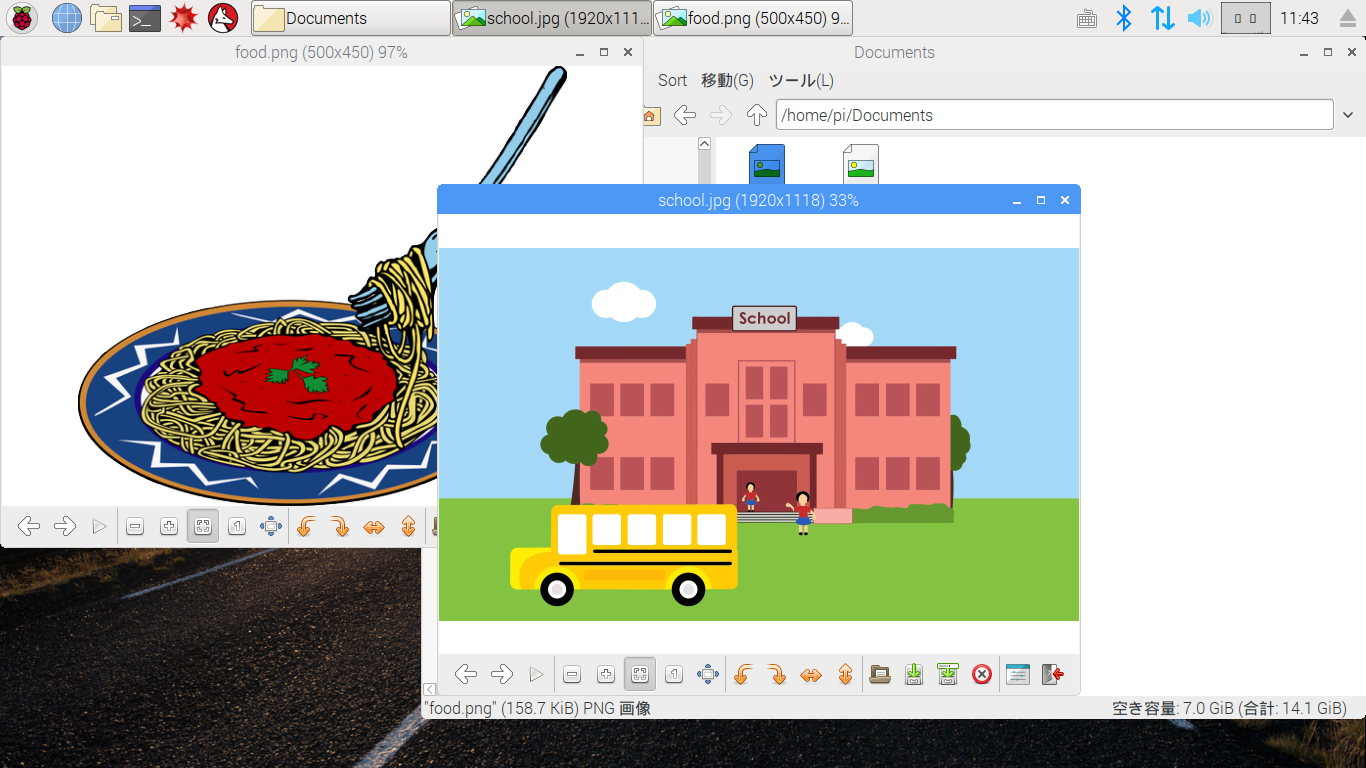
\includegraphics[width=0.65\textwidth]{text01-img/textbook-img221.png}
\flushleft

\bigskip


\subsubsection{\bfseries 問題 1-14 答え}



\centering
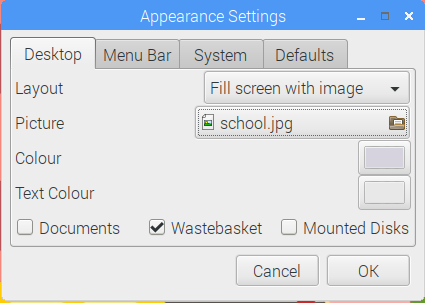
\includegraphics[width=0.55\textwidth]{text01-img/textbook-img222.png}


\centering
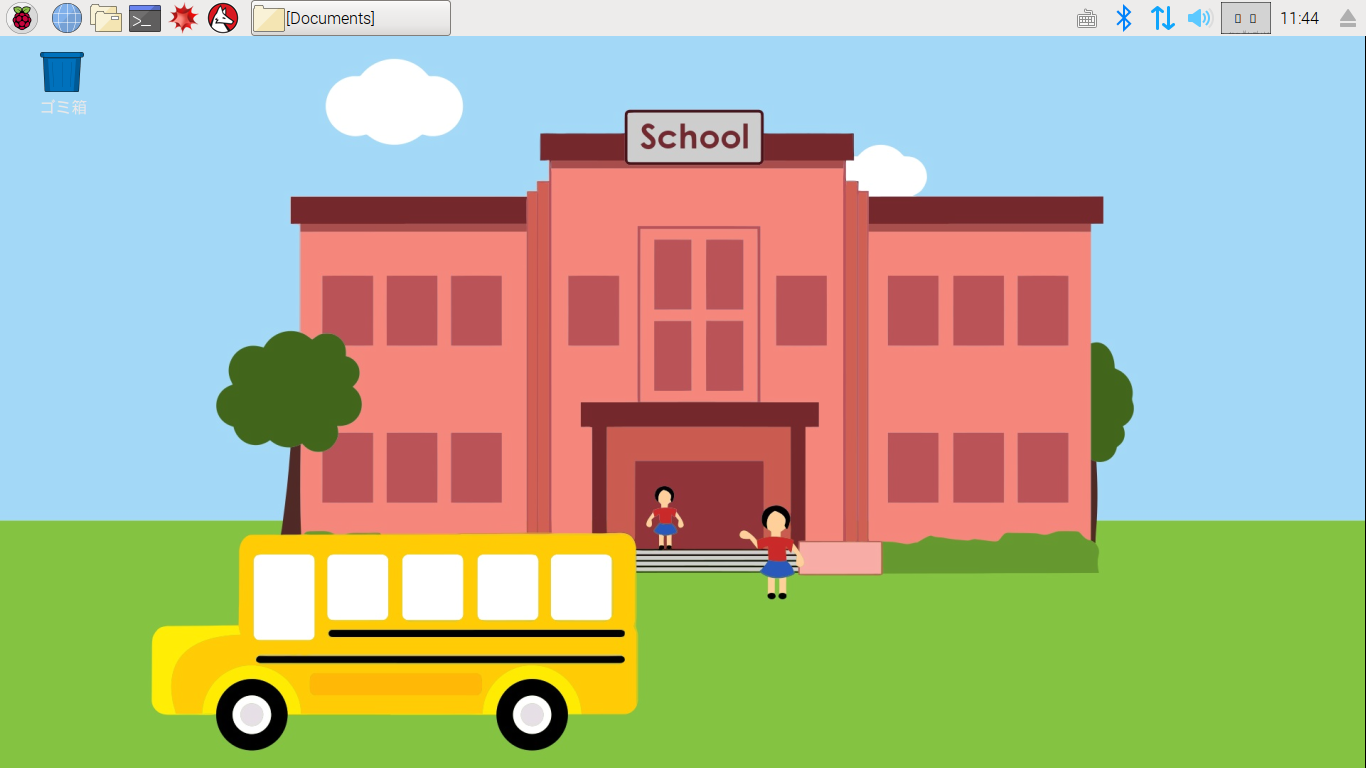
\includegraphics[width=0.65\textwidth]{text01-img/textbook-img223.png}


\flushleft
\clearpage
\begin{minipage}{\textwidth}
  \subsubsection{\bfseries 問題 1-17 答え}

  \centering
  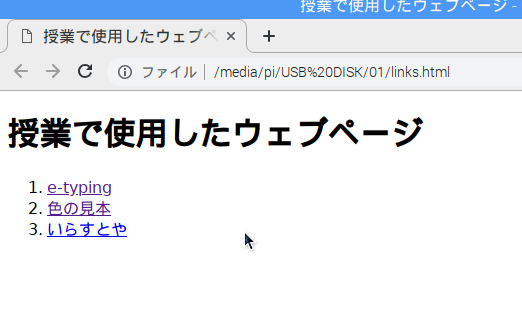
\includegraphics[width=0.4\textwidth]{text01-img/textbook-img224.png}
  \flushleft

  \subsubsection{\bfseries 問題 1-18 答え}
  % 表が入る
  \scalebox{0.8}{
    \begin{tabular}{ccc}
      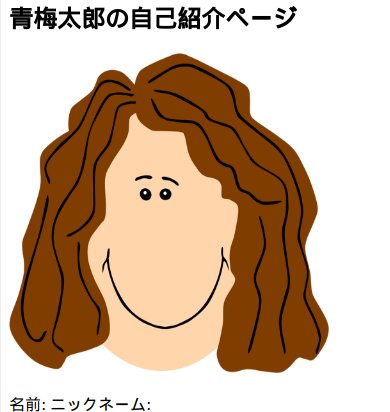
\includegraphics[width=5.373cm,height=5.579cm]{text01-img/textbook-img225.png} &
      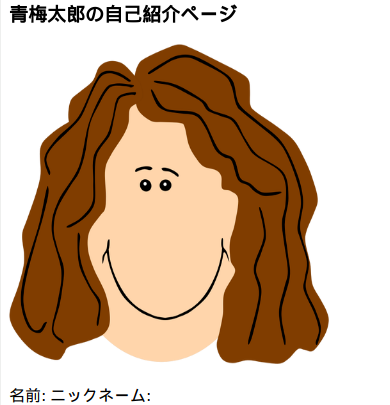
\includegraphics[width=5.373cm,height=5.579cm]{text01-img/textbook-img226.png} &
      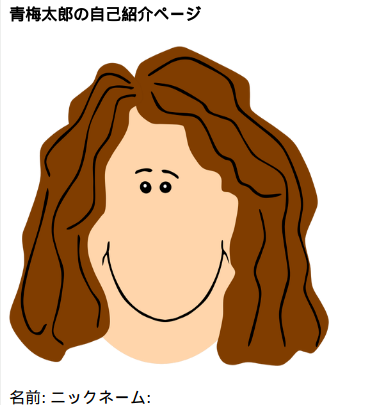
\includegraphics[width=5.373cm,height=5.579cm]{text01-img/textbook-img227.png}\\
      % \hline
      \large h2 &
      \large h3 &
      \large h4\\
    \end{tabular}
  }
  \vskip\baselineskip
  \scalebox{0.8}{
    \begin{tabular}{ccc}
      % \hline
      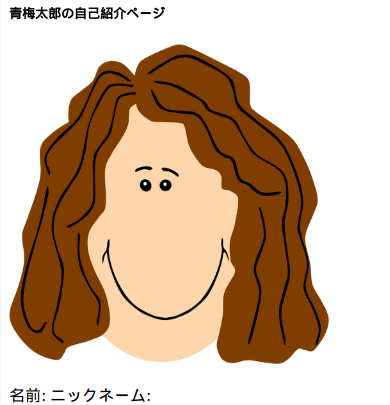
\includegraphics[width=5.373cm,height=5.579cm]{text01-img/textbook-img228.png} &
      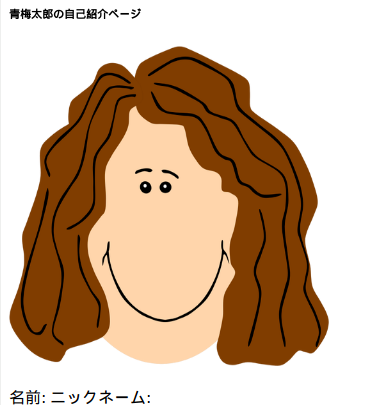
\includegraphics[width=5.373cm,height=5.579cm]{text01-img/textbook-img229.png} &
      ~\\
      % \hline
      \large h5 &
      \large h6 &
      ~\\
      % \hline
    \end{tabular}
  }
  \vskip\baselineskip
  h2〜h6にかけてじょじょに「青梅太郎の\ruby{自己}{じこ}\ruby{紹介}{しょうかい}のページ」の文字が小さくなっている。
\end{minipage}

\clearpage

\subsubsection{\bfseries 問題 1-20 答え}

\centering
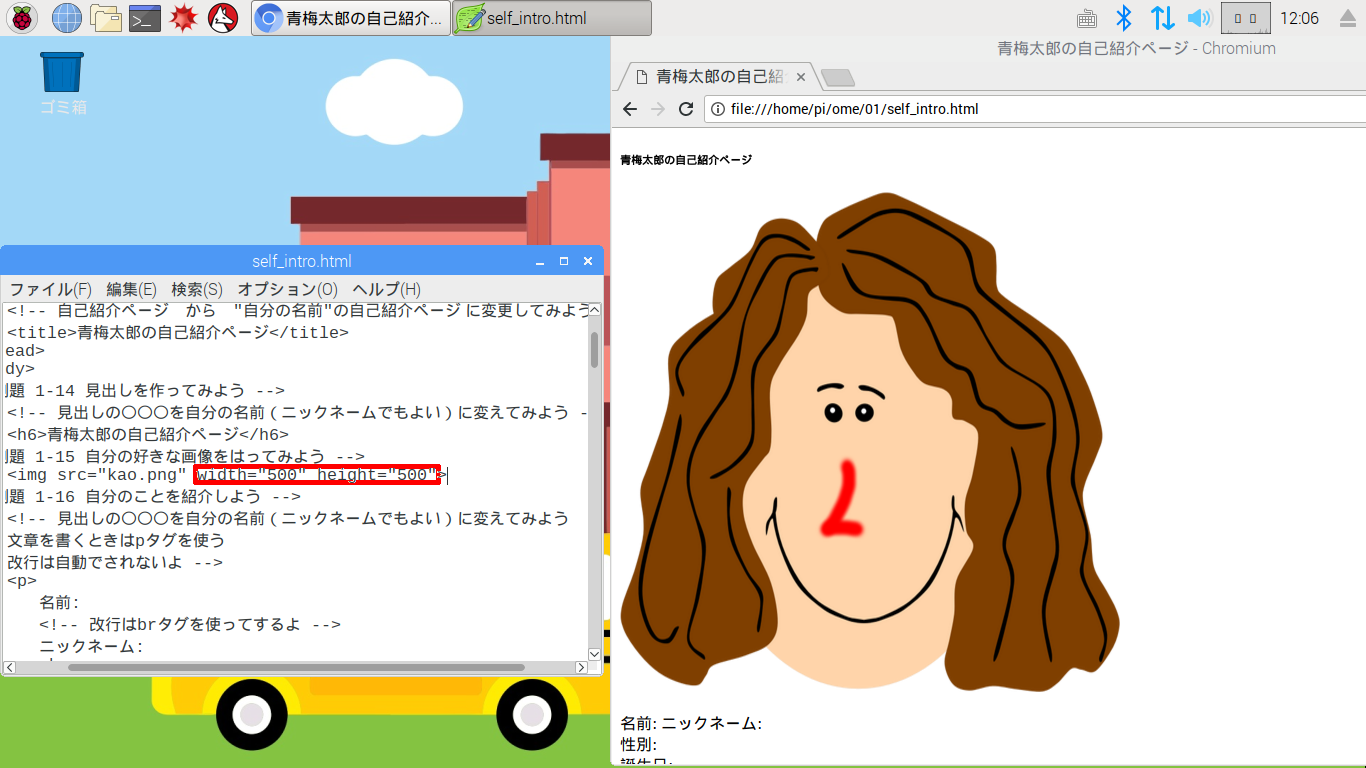
\includegraphics[width=0.65\textwidth]{text01-img/textbook-img230.png}
\flushleft
\ruby{画像}{がぞう}のサイズが変わっている。



\subsubsection{\bfseries 問題 1-21と問題1-22の答え}

参考にして自分のページを作ろう。

\fbox{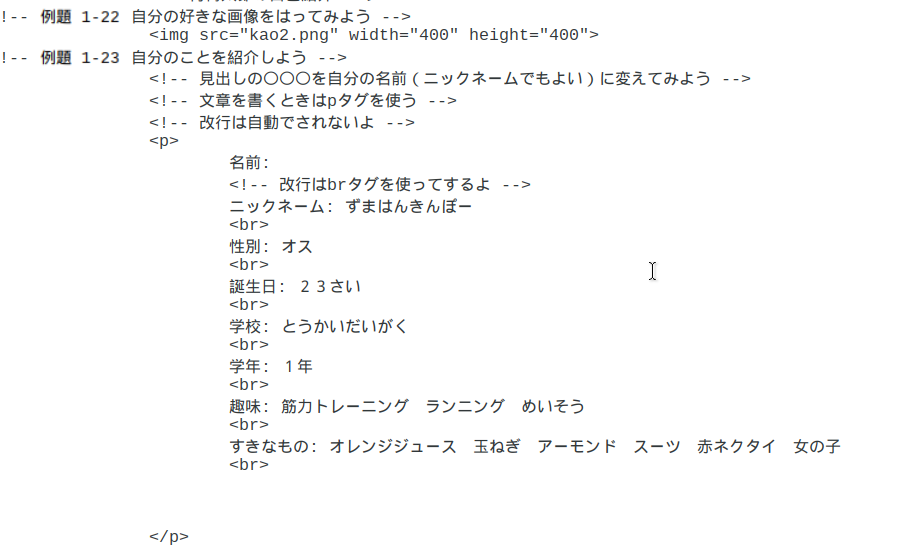
\includegraphics[width=0.65\textwidth]{text01-img/textbook-img231.png}}


\centering
\fbox{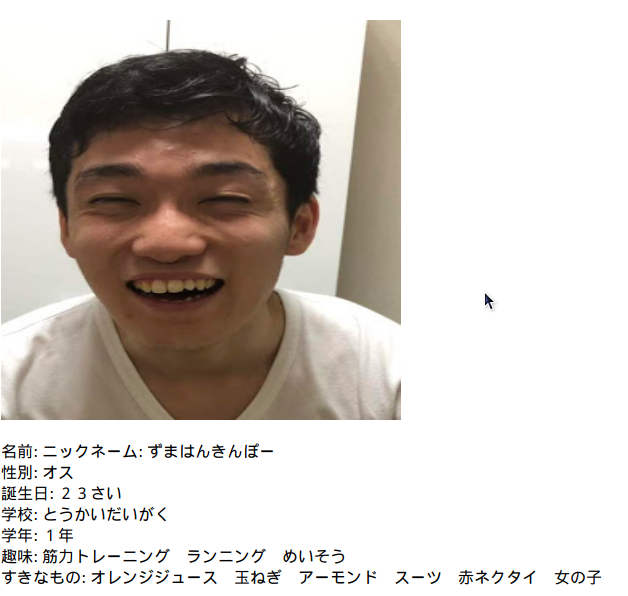
\includegraphics[width=7.354cm]{text01-img/textbook-img232.png}}


\clearpage

\flushleft
\subsubsection{\bfseries 問題 1-23 答え}

\centering
\fbox{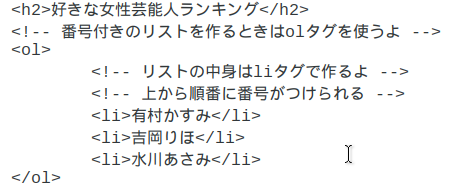
\includegraphics[width=8.245cm]{text01-img/textbook-img233.png}}
\fbox{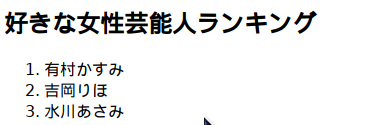
\includegraphics[width=7.422cm]{text01-img/textbook-img234.png}}
\flushleft


参考にして自分のページを作ろう。

\subsubsection{\bfseries 問題 1-24 答え}

ランキングではなく、\ruby{箇条}{かじょう}書きになる。

\centering
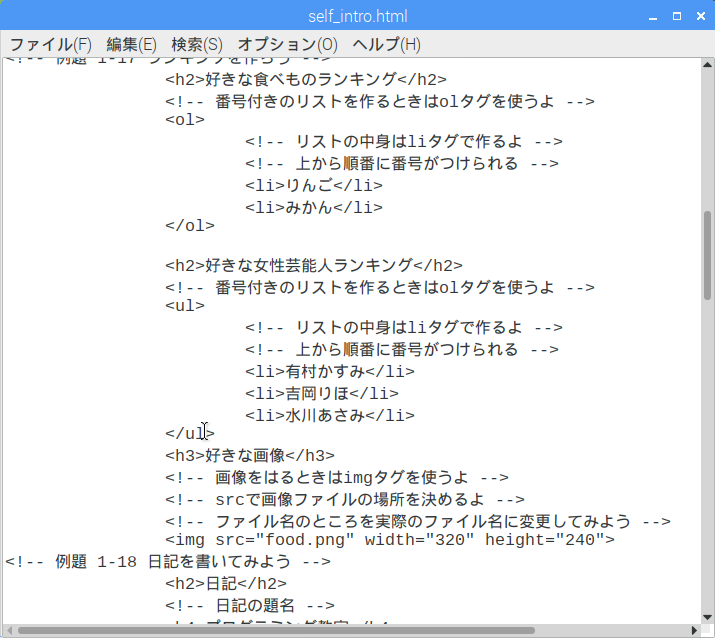
\includegraphics[width=7.622cm]{text01-img/textbook-img236.png}
\fbox{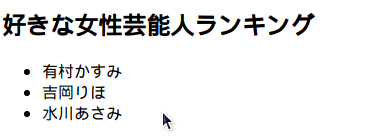
\includegraphics[width=7.904cm]{text01-img/textbook-img235.png}}
\flushleft

\bigskip

\subsubsection{\bfseries 問題 1-25 答え}

\centering
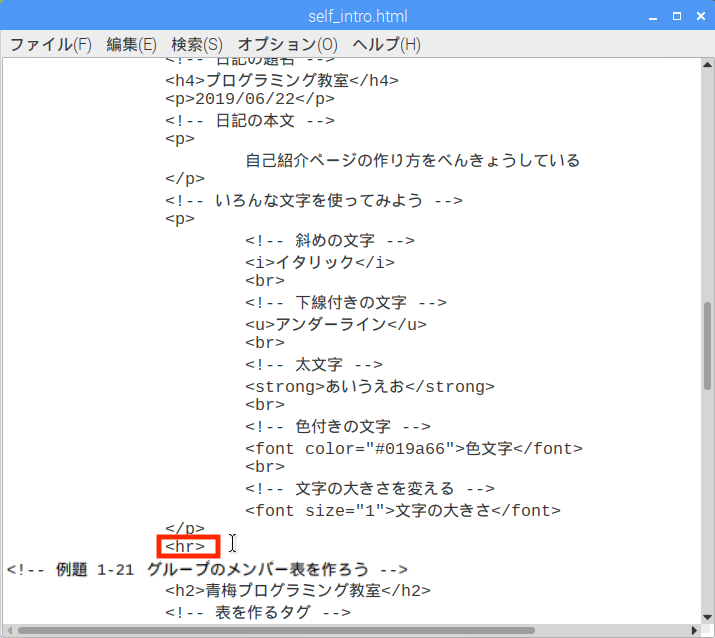
\includegraphics[width=8.186cm]{text01-img/textbook-img237.png}
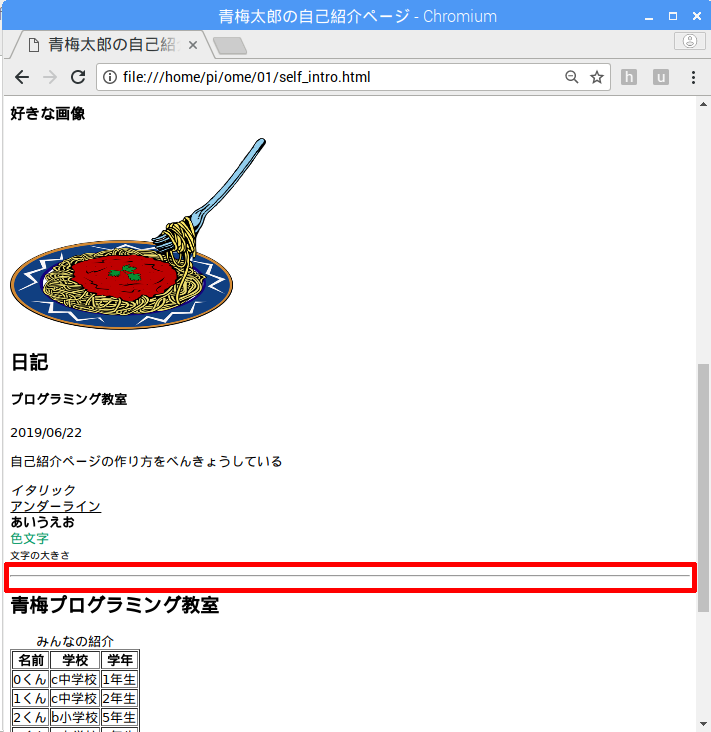
\includegraphics[width=7.163cm]{text01-img/textbook-img238.png}
\flushleft

\bigskip


\bigskip

\clearpage
\subsubsection{\bfseries 問題 1-26 答え}

\centering
\fbox{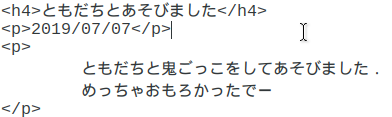
\includegraphics[width=9.938cm]{text01-img/textbook-img239.png}}
\flushleft

\bigskip

\centering
\fbox{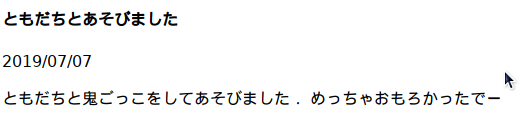
\includegraphics[width=0.9\textwidth]{text01-img/textbook-img240.png}}
\flushleft

\bigskip

参考にして自分のページを作ろう。


\bigskip

\subsubsection{\bfseries 問題 1-29 答え}

%\newline

\centering
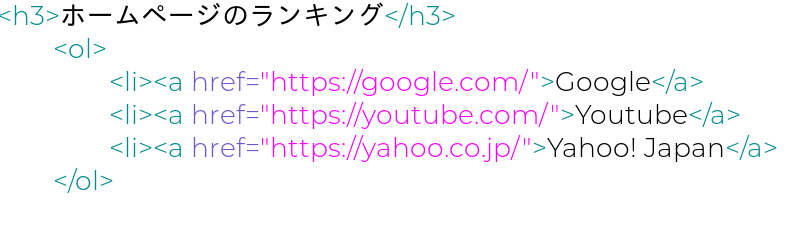
\includegraphics[width=0.8\textwidth]{text01-img/textbook-img241.png}
\flushleft

\bigskip

\centering
\fbox{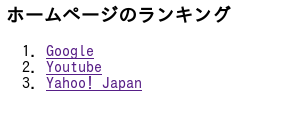
\includegraphics[width=0.5\textwidth]{text01-img/textbook-img242.png}}
\flushleft

\bigskip
参考にして自分のページを作ろう。

\clearpage
\subsubsection{\bfseries 問題 1-30 考え方}

%\liststyleLxxxii
\begin{enumerate}
  \item
        それぞれ\ruby{画像}{がぞう}をとります。35ページの例題1-16を参考にしましょう。
  \item リストの\ruby{項目}{こうもく}をliタグで追加します。
  \item
        liタグのしたにimgタグを追加して\ruby{画像}{がぞう}を\ruby{表示}{ひょうじ}します。55ページの例題1-22を参考にしましょう。
\end{enumerate}
\centering
\fbox{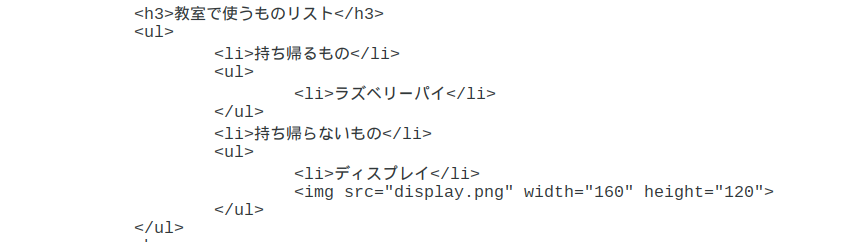
\includegraphics[width=0.8\textwidth]{text01-img/textbook-img243.png}}
\flushleft

\bigskip

\centering
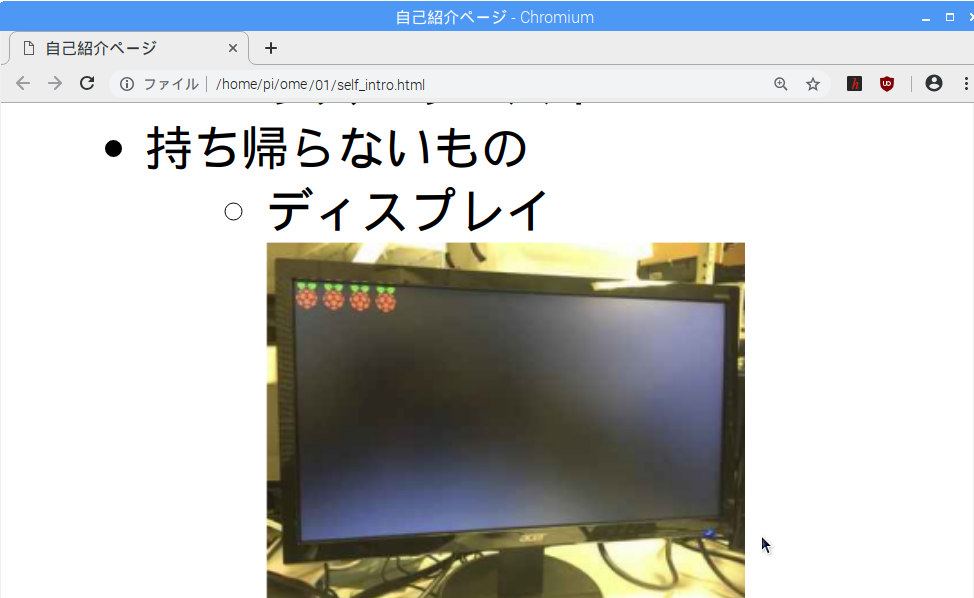
\includegraphics[width=\textwidth]{text01-img/textbook-img244.png}
\flushleft

\bigskip

\clearpage

